\documentclass[aspectratio=169]{beamer}
\usetheme{Madrid}
\usecolortheme{beaver}
\usepackage[utf8]{inputenc}
\usepackage[T1]{fontenc}
\usepackage{tikz}
\usepackage{amssymb}
\usepackage{graphicx}
\setbeamertemplate{navigation symbols}{}
\setbeamercolor{title}{fg=white,bg=cyan!60!black}
\setbeamercolor{frametitle}{fg=white,bg=cyan!50!black}
\setbeamercolor{block title}{bg=cyan!15,fg=black}
\setbeamercolor{block body}{bg=cyan!5,fg=black}

\title{Block Arcade 3 — Events}
\subtitle{Keys are events — the stage reacts to what the player presses}
\author{ByteForge --- Grade 7 --- Game Maker --- Week Overview}
\date{}

\begin{document}

\begin{frame}
    \titlepage
\end{frame}

\begin{frame}{This Week's Plan}
    \begin{itemize}
        \item Lesson 1: Press to Move
        \item Lesson 2: Jump on Space
        \item[$\bigstar$] BOSS --- Full Control (\texttt{lessonBoss.tex})
    \end{itemize}
\end{frame}

\begin{frame}{Real-World Example}
    \Large
    A car's cruise control constantly re-checking your foot on the brake, or a lift constantly checking if a floor button is pressed — both are "ask the same question every moment", not a one-time check. Minecraft's own WASD + Space controls are literally this chapter's pattern — each key its own independent check, which is exactly why you can strafe (A/D) while jumping (Space) at the same time.
\end{frame}


\begin{frame}{Image}
    \begin{center}
    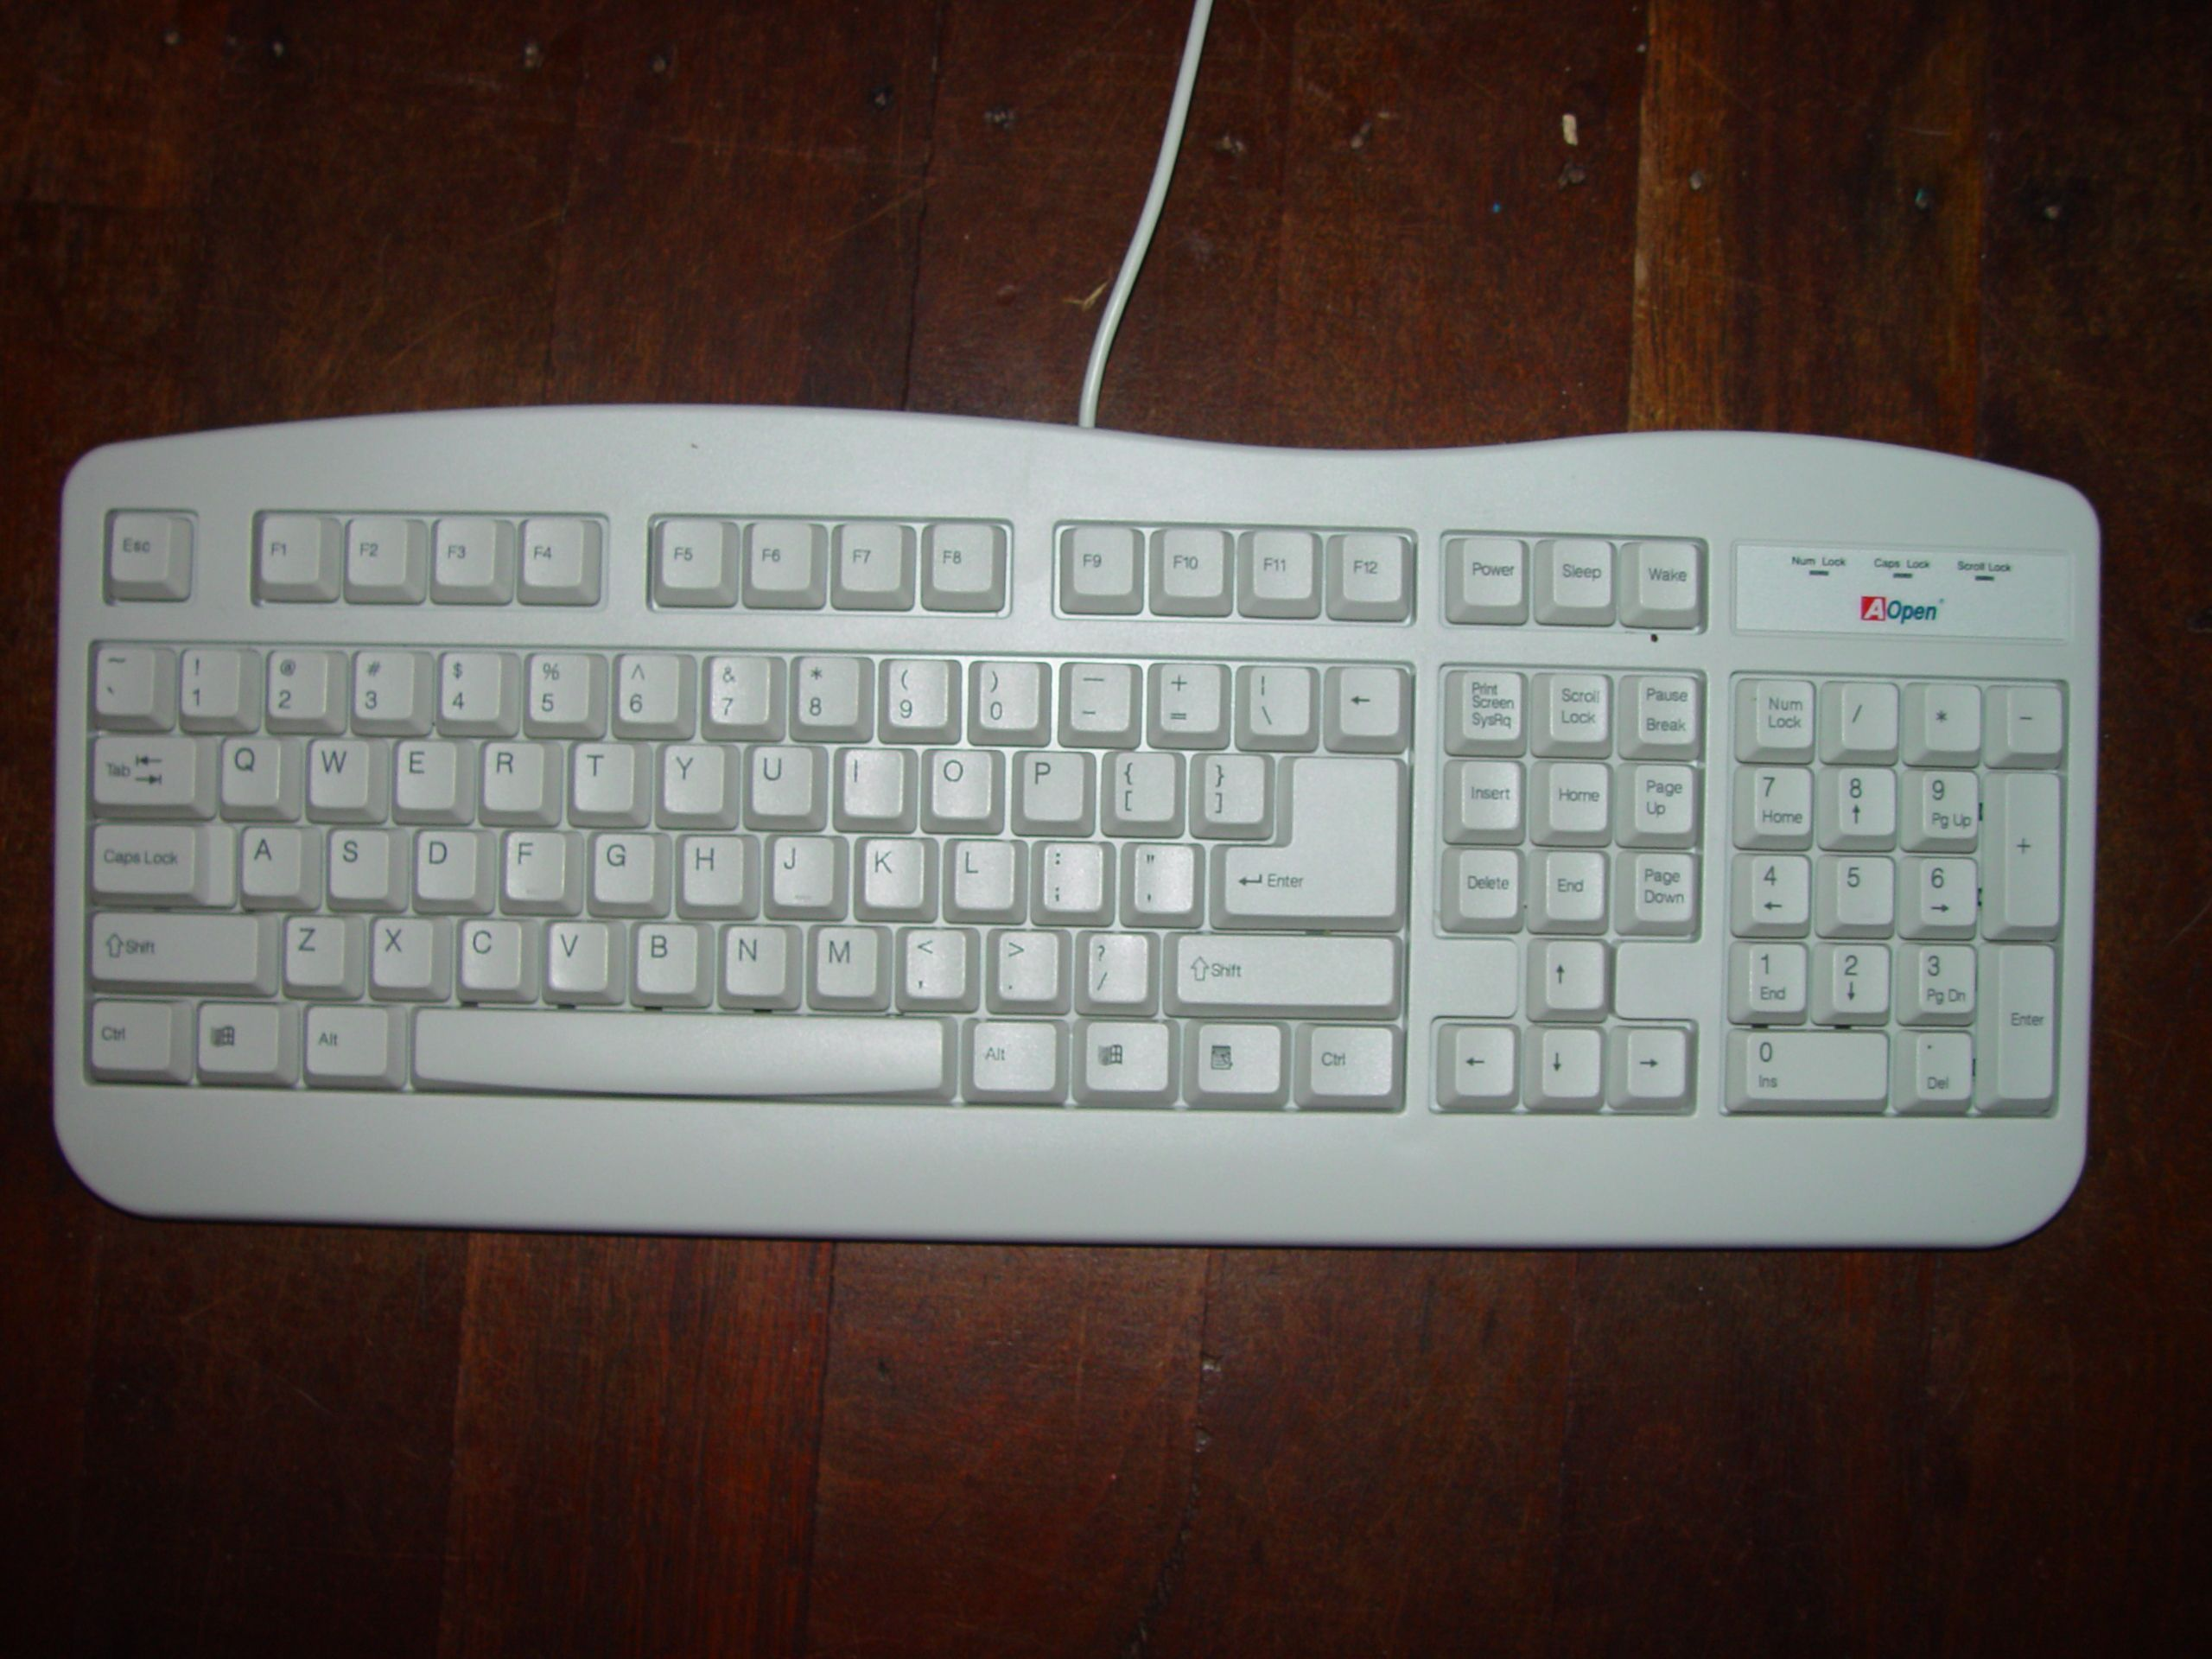
\includegraphics[width=0.55\textwidth]{../images/keyboard.jpg}

    \small Computer keyboard, public domain, via Wikimedia Commons
    \end{center}
\end{frame}

\begin{frame}{Let Them Discover}
    \Large
    Try holding two arrow keys at once in any real game (or your phone's on-screen d-pad), or W+Space in Minecraft. Does the character move diagonally / jump-forward? What would the code need to allow that — one if, or two separate ifs?
\end{frame}

\begin{frame}{Files in This Folder}
    \small
    \begin{itemize}
        \item \texttt{lesson1.tex} --- Press to Move
        \item \texttt{lesson2.tex} --- Jump on Space
        \item \texttt{lessonBoss.tex} --- BOSS: Full Control
    \end{itemize}
    \vspace{0.5em}
    \normalsize Each lesson file is its own short deck --- open the one for
    the specific day you're teaching, not this whole overview.
\end{frame}

\end{document}
